\documentclass{beamer}
\usepackage[utf8]{inputenc}
\usepackage[spanish]{babel}
\usetheme[secheader=true]{Madrid}
\useinnertheme{rectangles}
\usepackage{tikz}
\title[Memoria DDR]{Introducción a las Memorias DDR}
\subtitle[short subtitle]{long subtitle}
\author[msagre]{Miguel A Sagreras}

\date[2015]{}
%\institution[short name]{long name}
\begin{document}
\begin{frame}
\titlepage
\tableofcontents
\end{frame}

\begin{frame}
\frametitle{Primeras computadoras digitales}
\begin{tabular}{lll}
Año  & Nombre                & Observaciones \\
1938 & Torpedo Data Computer & Cálculo del disparo de torpedos\ 
	kdkdkdkd
1941 & Zuze                  & Cálculo del disparo de torpedos\\
\end{tabular}
\end{frame}


\section{Memoria de un transitor por bit}
\begin{frame}
\end{frame}

\begin{frame}
\begin{figure}[!htb]
\centering
\includegraphics[scale=1.0]{membank.eps}
\end{figure}
\end{frame}

\section{Banco de Memoria}
\begin{frame}
\begin{figure}[!htb]
\centering
\includegraphics[scale=1.0]{chip.eps}
\end{figure}
\end{frame}

\section{Secuencia de acceso}
\begin{frame}
	\begin{itemize}
		\item Acceder a la fila
		\item Acceder a la columna
		\item Recuperar el valor leido
	\end{itemize}
\end{frame}

\section{Timing diagram}
\begin{frame}
\begin{figure}[!htb]
\centering
\includegraphics[scale=1.0]{dram-timings.eps}
\end{figure}
\end{frame}

\section{Timing diagram}
\begin{frame}
\begin{figure}[!htb]
\centering
\includegraphics[scale=1.0]{ddrdram-timings.eps}
\end{figure}
\end{frame}

\section{fpga}
\begin{frame}
\begin{figure}[!htb]
\centering
\includegraphics[scale=1.0]{fpga.eps}
\end{figure}
\end{frame}

\end{document}

